\subsection{Worked Example}
\label{sec:converter-example}

The converter of the example station at its operating point of Section~\ref{sec:station-example} has
$U_{valve} = \cvUv$\,kV, $P_{ac} = \cvP$\,MW, $Q_{ac} = \cvQ$\,Mvar and $U_{dc} = \cvUdc$\,kV. The arm
currents are $I_{arm\_rms} = \cvIrms$\,kA and $I_{arm\_peak} = \cvIpk$\,kA. Figure~\ref{fig:converter-arm} shows the arm voltages,
the arm currents and the capacitor voltages of phase a over one period; Table~\ref{tab:converter-losses} gives the
losses of the detailed model and Table~\ref{tab:converter-capacitors} the capacitor quantities.

\begin{figure}[!ht]
  \centering
  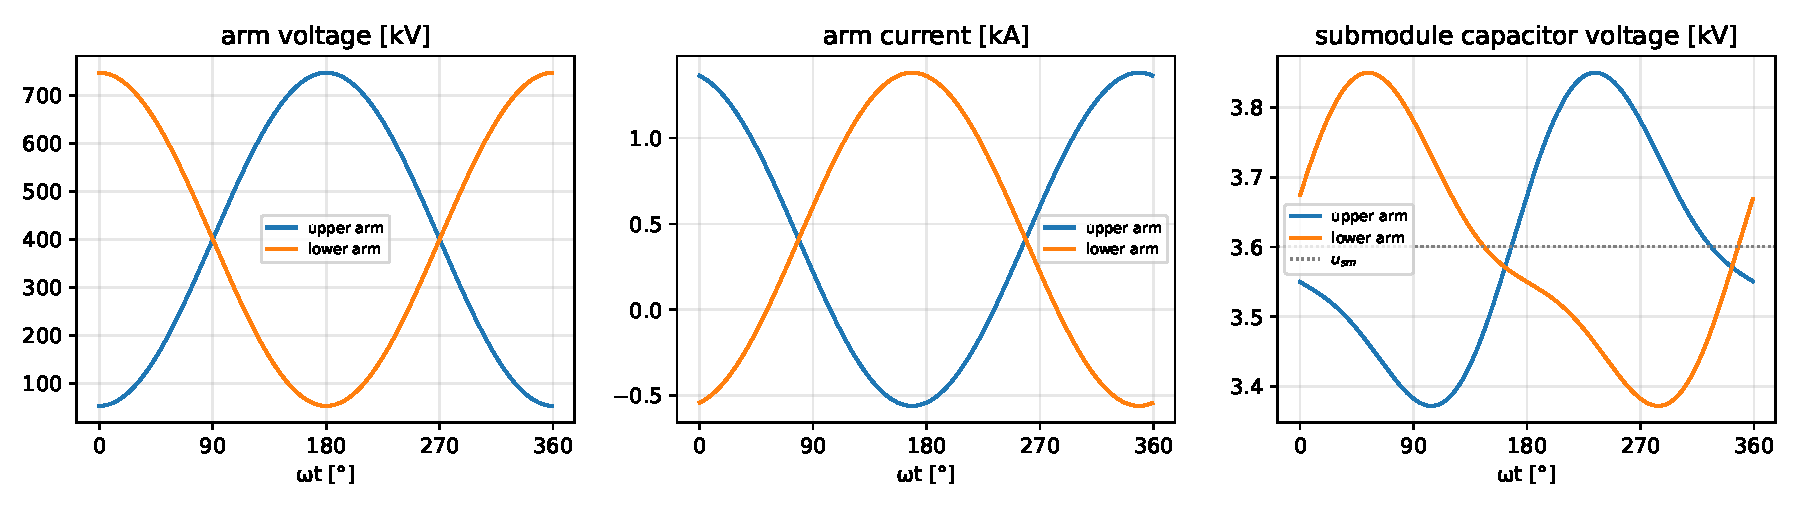
\includegraphics[width=\linewidth]{converter/fig/arm_waveforms.pdf}
  \caption{Arm voltages, arm currents and submodule capacitor voltages of phase a over one period, converter of the
           example at $P_{ac} = \cvP$\,MW (rectifier)}
  \label{fig:converter-arm}
\end{figure}

\begin{table}[!ht]
  \centering
  \small
  \begin{tabular}{@{}l r r@{}}
    \toprule
    \textbf{Part} & \multicolumn{1}{c}{\textbf{MW}} & \multicolumn{1}{c}{\textbf{\% of $|P_{ac}|$}} \\
    \midrule
    \tablerows{converter/fig/losses_table}
    \bottomrule
  \end{tabular}
  \caption{Converter losses of the example, loss model \texttt{detailed}, two modules in parallel}
  \label{tab:converter-losses}
\end{table}

\begin{table}[!ht]
  \centering
  \small
  \begin{tabular}{@{}l r l@{}}
    \toprule
    \textbf{Quantity} & \multicolumn{1}{c}{\textbf{Value}} & \multicolumn{1}{c}{\textbf{Unit}} \\
    \midrule
    \tablerows{converter/fig/capacitor_table}
    \bottomrule
  \end{tabular}
  \caption{Modulation and submodule capacitor quantities of the example, $C_{sm} = 3.7$\,mF}
  \label{tab:converter-capacitors}
\end{table}
\FloatBarrier
